\subsection*{\textcolor{subsectioncolor}{\textsf{8. \textit{STATE DIAGRAM}}}}
\addcontentsline{toc}{subsection}{8. \textit{STATE DIAGRAM}}

%Menggambarkan proses yang dilaksanakan sistem, memuat:
%- state
%- state variable
%- action

\includegraphics[width=0.3\textwidth]{DiagramKeadaan}

\begin{description}
\item[$S_{0}$] adalah keadaan menganggur (menunggu masukan).
\item[$S_{1}$] adalah keadaan menanggapi. Pada penerapannya, keadaan ini mencakup menampung masukan ke dalam penyangga, mengolah tiap masukan yang ada di penyangga, dan memberikan keluaran.
\item[$0$] adalah tindakan tidak menerima masukan apa-apa. Untuk keadaan $S_{1}$, hal ini merupakan tidak adanya masukan yang harus diolah lagi di penyangga.
\item[$1$] adalah tindakan menerima masukan (misalnya untuk masukan teks, pengakhiran masukan ditandai dengan \textit{carriage return} dan/atau \textit{line feed}).
\end{description}
